% 来源：OEBPS/Text/Section0001_split_004.xhtml#sigil_toc_id_33

\BookChapter{22}
\section[第22章\q 终极目标清单：资产配置]{第22章\\ 终极目标清单：资产配置}

\begin{BookQuote}
试探河水有多深，千万不要两只脚都伸进去。

\hfill ——沃伦·巴菲特
\end{BookQuote}

假使你的赚钱机器就要启动了，可万万没想到你的老板突然给你发了1万美元的奖金，或者你突然得到了一笔10万美元的遗产。拿到了钱，你当然非常开心，可是，你用这样一大笔钱干什么？把钱放进你的银行储蓄账户，或者你的个人退休金账户吗？投资几个虚拟的比特币吗？在亿贝上投标一箱精制葡萄酒吗？买上100股苹果公司的股票吗？你把所有的钱都投资到一个地方，还是分散投资呢？

你怎么回答最后这个问题，是决定你财务未来的关键。

资产配置是你一生最重要的投资决策，比你做的任何一项投资决策都重要得多，不管你投资股票、债券、房地产或者其他东西。它的影响有多大？你已经做出了财务决策——自动地从你的收入中拿出一定比例用于投资来获得复利收益，这让你进入投资游戏。但是，一旦你决定进入这个投资游戏，你就会待在这个游戏里很长时间！如果你不小心谨慎地、仔细地选择你的投资方向，你就会把这些钱都输掉。任何人都能变得富有，资产配置决定你能保持富有。

但是你不要只相信我说的话。我们来听机构投资界的明星戴维·斯文森讲一讲如何做好资产配置。你要知道，他把耶鲁大学的捐赠基金投资组合从1亿美元做到了超过239亿美元，过去30年，即使经历了牛市和熊市，他也获得了13.9\%的年化收益率。业绩做到如此优异，真是无人能比。我和戴维·斯文森在他位于康涅狄格州纽黑文市的办公室里，面对面地交谈。我问他：“投资者要获得财务自由，必须拥有的投资工具是什么？”他告诉我，只有三种工具能够降低你的风险，增加你获得财务成功的潜力。

1.证券选择——挑选股票。

2.市场择时——短线选时，就是赌市场短线是涨还是跌。

3.资产配置——分散投资的长期策略。

在我还没有问前面两个工具前，他就讲：“在这三个工具中，最重要的是资产配置，它具有压倒性优势。在投资界，资产配置事实上的投资收益超过100\%。”等一下，怎么可能会超过100\%？因为交易会发生费用、税收、亏损，你做选股或者择时都会增加费用和税收。选择失误就会亏损，减少你的盈利。

资产配置不仅是分散投资，而且要把你的钱分开，分别投入不同种类的资产或者不同类型的资产（比如股票、债券、大宗商品、房地产）中，你要提前决定具体的投资比例。这取决于你的目标、需要、风险承受力、人生阶段。

这话是不是说得太大了？

在金融市场这个巨大的赛场上，对于世界上最优秀的选手来说，包括我在本书中采访过的每一位投资者和交易者，成功和失败的关键在于资产配置。保罗·都铎·琼斯就极其依赖资产配置。玛丽·卡拉汉·厄道斯可以称得上证券投资界最有权势的女人，领导着22000名金融专业人士，这些人赚钱养家全靠资产配置。瑞·达利欧创建了全球最大的对冲基金，现在他的个人财富高达140亿美元，他也全靠资产配置。

这一章讲的是一个复杂的主题，我要讲得非常简单，简单到足以让你能够照着去做，以期对你余生的投资收益产生积极的影响。所以你要对资产配置全身心投入，用全部精力来关注！不管你是打算积攒1000美元做投资，还是打算积攒100万美元做投资，资产配置都同等重要。你学到的这些原则至关重要，你要马上开始运用。如果你觉得自己已经知道这些原则了，那么你要进一步深入地理解并实践应用，把它提升到更高的层次。

我们来谈一谈，为什么资产配置对你的投资计划如此重要，以及你如何今天就开始让资产配置为你工作。

\begin{BookQuote}
谁要是觉得数据安全，那他肯定没有看过报纸上的股票市场行情版。

\hfill ——艾琳·彼得
\end{BookQuote}

你到超市购物，排队付款，有多少次你选了看起来最快的队伍，结果反而成了最慢的那一队？或者你开车遇到堵车，你换到那条看起来更快的车道，结果却看到原来那条拥堵的车道上，车辆从你身边飞过呢？你觉得变道能更快些，结果你完全错了。夫妻关系不也是这样吗？不管你对自己多么了解，不管你多么相信对方，看重对方，你还是选择了“错误的”人生伴侣？我们都知道，这个选择特别重要，会对你一生的生活质量产生巨大影响！

同样的事情也会发生在你的投资上。一般的投资也就算了，你要是在养老金投资上出现错误，而且是一个大错误，那一切都完了。这意味着你连住的房子都保不住了。你可能都70岁了，还要去找工作，不干活就没饭吃。也可能你没钱给孩子交学费了，孩子的前途就这样完了。正是因为这个原因，这一章特别重要。

资产配置是一项关键的投资技能，有了这一技能，你就能超越其他99\%的投资者，从此鹤立鸡群。你肯定想不到，做资产配置有这么大的好处，却不会花费你一分钱。戴维·斯文森喜欢引用哈里·马科维茨的话。马科维茨曾获得诺贝尔经济学奖，也是现代投资组合理论之父，我也采访过他。马科维茨说过一句话非常有名：“分散投资是唯一免费的午餐。”为什么？因为把你的钱分散到不同投资上，长期而言，能减少你的投资风险，同时提高你的潜在收益，而这样做不会花费你一分钱的成本。

我们都曾经听过那句古老的谚语：“不要把所有的鸡蛋放在同一个篮子里。”是的，资产配置可以保护你避免犯下那种投资理财的错误，这听起来像是一个基本原则，但是你知道有多少人违反了这个投资的基本原则吗？

我有一个朋友，非常看好苹果公司，一提到苹果公司就非常兴奋、激动，他把他所有的钱都投到苹果公司这一只股票上。曾经有一段时间，苹果公司的股票成了世界上最牛的股票，但是几个星期后它就暴跌了40\%。我还有另外一位朋友，30多岁了，原来在一家电视台做高管，她辞职了，卖掉了洛杉矶的房子，正好是在房地产市场大牛市的最高点，她赚了很多钱，并用这笔钱在怀俄明州开了一家小餐馆。她把剩下的钱投在高风险股票和垃圾债券上，她认为只是这些债券的利息就足够支撑她的日常花销了。有几年确实如此，但是2008年爆发金融危机，股票暴跌，债券也暴跌，她一下子亏光了所有的积蓄，她不得不关掉小餐馆，重新回去工作。她成为一个自由职业者，很辛苦，但收入只有原来的一小部分。

\subsection{一定要分散}

我们都听说过经济危机期间发生的那些非常恐怖的事情。也许你知道婴儿潮世代中的有些人把所有的钱都投到了房地产上，结果正好赶上房地产大崩盘。有对夫妻就要退休了，他们的401(k)账户里已经存满了钱，他们的目标日期基金马上就要到期了。他们选好了一辆房车，旅行路线也规划好了，把中途去看望孙子的时间地点都标好了，但是后来金融世界崩溃了，他们的投资净值一下子减掉了将近一半，享受退休生活的美梦变成了还要再工作20多年。

\begin{figure}[htbp]
\centering
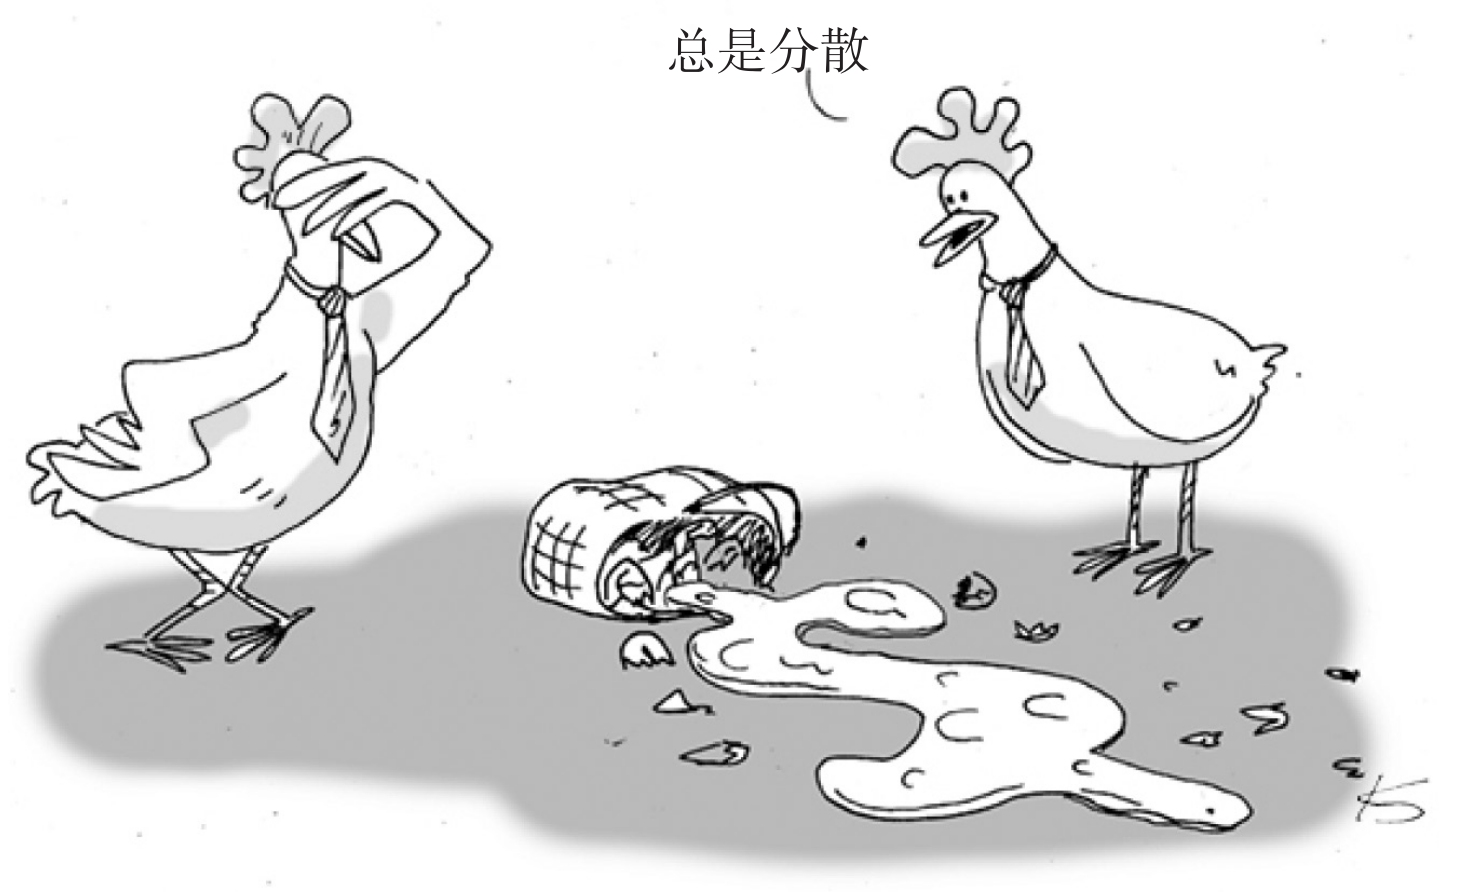
\includegraphics[width=0.76\linewidth,keepaspectratio]{image/22-1.jpg}
\caption{}\label{fig:22-1}
\end{figure}

这些故事令人心碎，我想确保这种事不会发生在你身上。好消息是，这种事并非必然是如此结局。这正是我要写本章的原因：你不但能够保住自己用来养老的财富，还能让你的这些养老金投资升值得更快。

这里简单又关键的投资教训是什么？那些现在涨的投资，将来肯定会跌。瑞·达利欧直截了当地告诉我：“几乎可以确定的是，不管你把你的钱投到什么上面，将来都会遇上大跌的日子，让你亏损50\%\textasciitilde{}75\%。”这意味着你选择的任何投资都有可能亏掉1/2\textasciitilde{}2/3，为什么大多数人会偏爱一种类型的投资？因为他们觉得自己对这方面更“了解”，或者因为现在这类投资有热门的回报，有些人倾向于把他们所有的钱都投到房地产上，有些人倾向于全部投到股票或者大宗商品上。如果没有足够分散，你就可能亏掉内裤！你听清楚我说的了吗？不管你计划得多么好，任何一种类型的资产，将来都可能和你算总账。所以，你只有两条路可以选择，要么分散，要么亏损。但是，如果分散投资做得好，你就会赢。

到现在为止，我可以肯定，你非常清楚不做分散投资，后果会非常严重！现在你愿意听我讲把分散投资做好了，效果会好到不可思议吗？这就像是拿到了许可，你能随便印钱一样。我知道，这么说有些夸张，但是想象一下，即使你在睡觉，你也照样能够赚钱。做好了分散投资，你的内心会非常平静，无论经济形势怎么变化，你都不用担心。

这里有个真实的案例。在2008年金融危机的经济形势下，股市跌了接近2万亿美元，债券市场也跌得很惨，房地产价格都跌到了谷底，你持有一个分散的资产组合，最多也只亏损3.93\%，你会感觉怎么样？这个案例并不是幻想出来的，而是真实的。这就是资产配置的威力，我在本书里已经提过好几次，我将很快证明给你看。1984—2013年，你的资产配置如此强大，以至你只有4年亏损，平均亏损比例为1.9\%，亏损最多的年份也没有超过3.93\%。记住在这些年里，其他人的财富都随着通货膨胀和通货紧缩的狂潮起伏不定。在最近十年中，我们就遇到过两次股市暴跌，接近腰斩，但是你会继续安全航行，穿越这些风暴，不需要考验你的胆量，你仍然能够平均获得接近10\%的年化收益率。我描述给你的是一个真正的投资组合，一个明确的资产配置，它由瑞·达利欧设计，我很快就会向你展示这个具体的资产配置公式。正是这个公式创造出令人非常兴奋的投资业绩。但是在实际运用它之前，你必须明白资产配置的核心原则，这就是我们这一章要展开论述的内容。


\begin{BookQuote}
第一条，不要亏本。

第二条，记住第一条。

\hfill ——沃伦·巴菲特的投资法则
\end{BookQuote}

再强调也不过分：好人经常失败，因为尽管他们做的事是正确的，但他们做事的时间是错误的。买套房子，是不是正确的事情？大多数专家会说“是的”，但是在2006年买房是一个错误的时机！所以问题是，如果我们无法避免犯错，那么我们应该把钱投到什么地方。这就要发挥资产配置的作用了。

还有另外一种思考方式：如果你正在努力打造一支球队，想让它获得胜利，你必须知道球队中每个队员的能力，以及每个队员的强项和弱项。你必须决定，在不同的情况下，你可以依靠谁。现在打个比方，你的投资组合就是一支球队，你的投资选择就是队员，资产配置帮你选择由谁先发，它在什么位置。最终，在正确的时候，用不同的球员做正确的组合，这才能给你带来胜利。

资产配置给你提供了一套指导原则，这种投资哲学帮助你决定你的自由基金或者养老金投到了什么地方，它们各占多大比例。

你可以想象，把你的钱分别放进两个不同的投资水桶里，每个水桶的风险水平和收益水平不同。第一个水桶是给你的钱打造一个安全的环境，但是钱在这个水桶里增值得非常慢。你也许会觉得财富增长这么慢，一点儿意思也没有，但是你的钱很安全，当你需要钱的时候，钱肯定在那里，一分也不会少。第二个水桶的吸引力要大多了，因为它能给你机会获得更快的财富增长，但是高收益背后是高风险。事实上，你必须做好准备，把钱投到这里有可能亏得精光。

每个水桶该放多少钱？这取决于你有多少时间来让你的投资增长，以及你愿意承受多大的风险。你需要问自己：“在我生命的这个阶段，我能承担多大的风险？”请记住，你做分散投资，并不只是为了保护自己。你希望能够强化自己的业绩，找到各种投资的理想组合，这能够让你茁壮成长，而不仅是维持生存。

但是如果我们愿意承认的话，很多人的生活压力其实已经非常大了，根本承受不了因为投资而再增加的一大堆忧虑。财务安全甚至财务自由很大程度上意味着一份内心的平静，让你觉得自己不用再为钱担心了。第一个水桶给你带来人生的确定性，毕竟确定性是人类的第一大基本需要。我称之为安全/安心水桶，有了确定性，你就安全了，也能安心了。这个水桶用来放未来养老的钱，你亏不起，甚至一想到这些钱要亏掉，就会惊出一身冷汗，半夜都会惊醒。这是个避难所，只做安全的投资，你要紧紧锁定，确保安全，甚至连钥匙都要藏起来。

\begin{BookQuote}
我不赌博，因为赌赢100美元并不能给我带来很大的快乐，但是要输掉100美元，会把我气疯。

\hfill ——艾利克斯·特里贝克（《危险边缘！》节目主持人）
\end{BookQuote}

财务损失不只会让我们的钱包缩水，还会偷走我们生活的快乐。你还记得那个关于猴子和苹果的行为经济学研究吗？给猴子一个苹果，他很快乐，但是如果你给猴子两个苹果再拿走一个，那它就发火了——尽管最终结果是一样的，它手里还会有一个苹果。人其实也一样。关于人类情绪的研究表明，世界上大多数人都低估了他们遭受损失时的糟糕感觉。胜利给我们带来的快乐，远远比不上失败或者损失给我们带来的痛苦。所以我们必须设立一个安全/安心水桶，来保护我们自己，避免自己承受这种打击。这样的打击不只让我们的财富缩水，而且让我们感觉非常痛苦。

为了让你对这类投资更加熟悉，我们先来看一下8种基本类型的资产（投资选择或者投资资源），它们应该属于这种安全/安心水桶。这里只是举例说明，并不意味着每种投资都适合这个水桶。但是，你在阅读的时候，会注意到一种模式：这些类型的投资一般都没有强烈的波动性。这意味着这些投资的价值不会有什么大的波动，特别是和你在风险/成长水桶里看到的那些投资相比。（不过，在历史上一些短暂的时期，几乎所有投资的波动性都会提高，后面瑞·达利欧会给我们展示如何做好准备，防范这种极端情况。）这里有一个供你快速浏览的清单，目的是让你思考你的投资未来。问问你自己：“在我投资之前，这个投资会让我处于风险之中吗？这个投资放在我的风险/成长水桶里还是放在安全/安心水桶里，哪个对我更好？”

为了更好地回答这个问题，我们来看一看这两个水桶。我们先从第一个水桶开始，这也许是最重要的存放你的一部分钱的地方，这就是安全/安心水桶。你想把哪些资产放到这个水桶里？记住，安全/安心水桶里的投资增长很慢，但是很稳定，就像争取财务自由赛跑中的乌龟一样，而乌龟经常最终获胜。你需要把安全/安心水桶看作你的储蓄和投资圣殿，因为只要钱被放进去，它就不会再跑掉。

在你继续读下去之前，请牢记，这一章开始的一些基础知识：资产配置的基本操作。如果你是一个资深投资者，你只要浏览一下这些投资选项的清单就行了，因为你可能已经知道这些投资是什么了，你可以给自己节省一些时间。但是，我并不想抛下任何一个人，因为肯定有人对此一无所知。除此之外，你也许会发现，有一两项投资的特点是你以前不太了解的，它对你很有价值。

让我们开始吧。

1.现金和现金等价物。在我们人生的某个时候，每个人都需要现金来救急，或者突然有急事急需用钱，或者收入突然大幅减少不够花了。不管你的收入水平是高还是低，你都需要一些流动性，或者有办法马上拿到现金。你是否有这样的感觉，尽管在财产上很富有，但是你感觉很贫穷，因为你手上没有钱或者周转不过来？很多人在2008年都感觉手头很紧，因为银行的资金冻结了，停止了对外贷款，甚至银行之间也停止了相互贷款，房产好像根本卖不出去。事实上，根据2011年的研究，所有美国人里有接近一半的人很难一下子凑齐2000美元来应对危机，比如意料之外的医疗账单，打官司的钱，修理房子或修车的钱。所以，你需要一些现金，以保证这种既尴尬又难堪的事情不会发生在你头上。想一想，这并不需要你太多的注意力或者太多的储蓄，就可以让你比另一半美国人的日子过得更好。

但是，一旦你决定手头要留下部分现金，你会把这些现金放在哪里？我们大多数人会选择开设一个银行账户——由美国联邦存款保险公司做保险，提供的本金保障上限是25万美元的银行账户。不幸的是，那些实体银行近些年来基本不付利息。最近我查了一下，有些实体银行的存款利率低到只有0.01\%。虽然那些网上银行给的利率略高一点，但也只是高那么一点。也许利率不是那么理想，但至少我们知道钱是安全的，想拿就可以拿到。你也许想把这些救急用的钱拿出来一部分放到一个安全的地方，或者为了安全起见，就放在你的家里，比如“放到床垫下”，总之是一个安全的、隐蔽的地方，以防突然出现地震、飓风或者其他紧急情况，比如银行的取款机停止工作了，你账户上的钱取不出来。

其他可以作为现金等价物的投资工具包括货币市场基金，它有三种类型。如果你想了解更多，可以看一看下面的内容。

如果需要保证安全和流动性的资金数量比较大，你可以购买一些短期的投资产品，这叫现金等价物。其中最有名的就是历史悠久的货币市场基金。你现在可能已经拥有其中的一只了。货币市场基金其实就是公募基金，只不过持有的都是风险很低、期限极短的债券和其他种类的债券而已（过一会儿我们会给你介绍更多的相关内容）。这些货币市场基金非常好，因为你得到的收益率要比令人厌烦的传统银行利息高出许多。你还可以享受每天24小时随时取现的便利，还有一些货币市场基金甚至可以让你开支票，和银行账户一样。

顺便说一下，大多数银行提供货币市场存款账户，这和货币市场基金不是一模一样的。它有点儿像存款账户，不过银行得到允许可以把你账户里的钱投到短期债务上，为此它们付给你稍微高一点的利息作为回报。这样的货币市场存款账户，通常有一个最低存款金额的要求或者其他限制，如果你的存款余额低于限额的话，银行会降低你的利率，还有一些惩罚措施。但是美国这种账户也由美国联邦存款保险公司提供保险，这是一件好事。这也是它们的特色，货币市场基金是没有保险的，你的投资价值可能会下跌，让你亏本。

如果你想“一举三得”，既安全又有流动性，还能够赚到利息，有一个选择是购买美国财政部货币市场基金，它有开支票的特权。美国联邦存款保险公司不为这种货币市场基金提供保险，但是因为它们只投资美国政府发行的国债，而不投资任何公司债或者银行债——这些企业发行的债券都可能违约，你亏钱的唯一可能性是美国政府违约，不能按期偿还短期债务。如果这种事情发生了，美国政府就垮台了，你所有的赌注也就赔光了！

2.债券。我们都知道债券是什么东西，对不对？我卖给你我发行的债券，就相当于我给了你一个承诺，我要说话算数。我买了你发行的债券，就是你给了我一个承诺，经过一定的时间之后（到期日），把本金还给我，再加上一定的利息。正是出于这个原因，债券也被称为“固定收益投资”。你能从这些债券得到的收益或者收入是固定的——你在买入的时候就知道得一清二楚，具体的收益率高低取决于你同意持有这些债券的时间长短。当债券到期时，你将获得一笔定期利息收益。所以债券就像一个简单的借条，钱不能白借，是有利益的，是不是？但是全球有数千万亿美元的债券和债券基金，虽然不是所有，但是大部分的债券都有评级，由不同的评级机构按照这些债券的风险水平给予信用评级。在本章的末尾，你会看到一个债券概述，你可以了解什么时候投资债券会严重危及你的财务健康，什么时候投资债券对你有利，甚至非常有用。

债券这种投资也会令人迷惑不解。就像跷跷板一样，利率下降时，债券的价值增加，利率上升时，债券的价值反而会降低。

\begin{figure}[htbp]
\centering
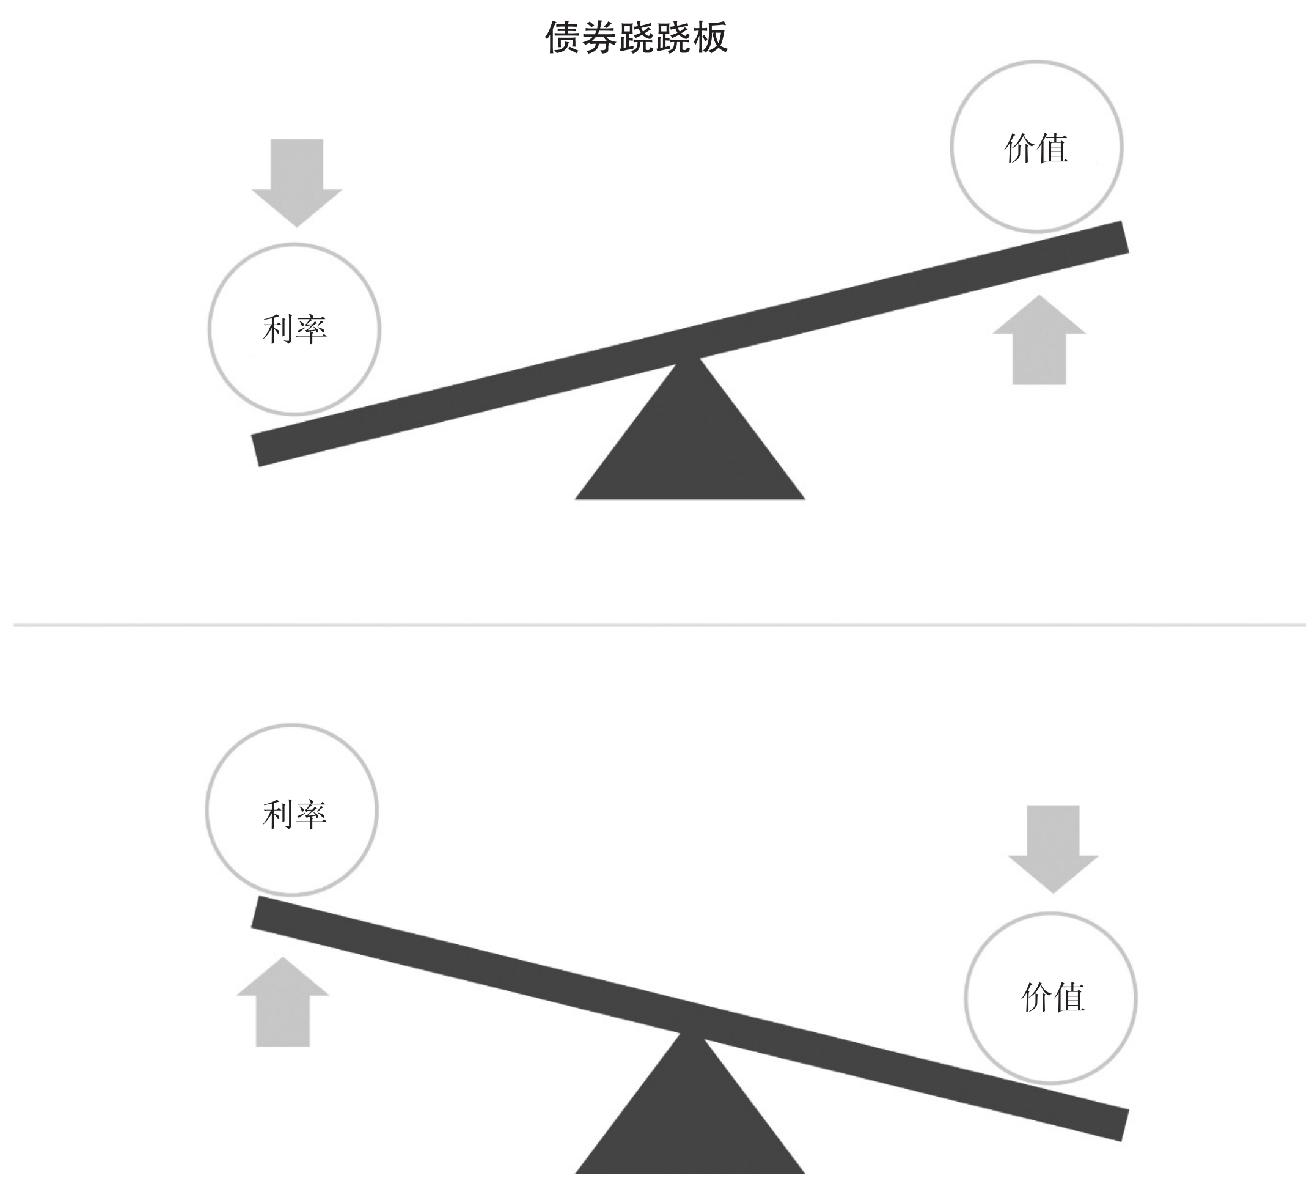
\includegraphics[width=0.64\linewidth,keepaspectratio]{image/22-2.jpg}
\caption{}\label{fig:22-2}
\end{figure}

毕竟，后面新出来的债券更有吸引力，利率更高，谁还会去买那些旧的、低利率的债券？但是有一个办法可以避免你担心的债券价格波动，那就是分散投资，购买低成本的债券指数基金。

只要记住，并不是所有的债券生来就是一样的。希腊的债券不像德国的债券那样强劲，底特律的市政债券不像美国联邦政府的债券那样稳健。事实上，有些投资顾问说，美国唯一安全的债券是由美国联邦政府完全以信用担保的债券。如果你真的能买到这样的美国债券，名称是美国财政部通货膨胀保值国债（简称TIPS），其价值与代表通货膨胀水平的消费价格指数保持同步。我们会在债券概述里面讨论这些内容。我会向你展示一个令人震惊的投资组合，并教你用非常独特的方式来运用债券基金。但是现在我们看一下其他的固定收益投资，也许它们可以列入你的安全/安心水桶。

3.大额存单。还记得大额存单吗？买大额存单，其实就是你借钱给银行。它们拿走了你的钱，付给你一个固定的利率。过完约定的一段时间之后，它们把本金还给你，再给你一笔利息。因为大额存单是由美国联邦存款保险公司承保的，所以它非常安全，和储蓄存款账户一样，就在我写本书的时候，它的收益率也一样让人提不起兴趣。但是我写本书是要帮你应对不同的投资季节，而季节是不断变化的。我不知道你现在所处的投资季节，但是我可以告诉你我的一个真实故事。1981年，那时我21岁，到银行就可以买一张6个月的大额存单，等到期的时候，我能拿到17\%的利息！17\%，太不可思议了！但是你不需要想太多就能明白，有些类型的大额存单在合适的环境下，能带给你高收益率。还记得我前面讲过的那个故事吗？我在堡垒投资理财公司的财务顾问在2009年给我提供了一个大额存单，固定收益率相当低，但这是一个市场联结型的大额存单，和股市涨幅挂钩，因此它给我们创造了8\%的平均收益率！这是一笔非同寻常的好买卖，但是还有其他一些方法可以被用来投资这些市场联结型的存单，它能为你创造更高的收益（却并不用让你的本金承担风险）。

我们上述这些不同类型的资产所组成的团队到现在为止表现得怎么样？大额存单、现金、货币市场基金、债券，这些资产选手明显适合进入你的安全/安心水桶。但是什么时候你派它们上场比赛？有些选手在某些情况下表现得很好，但在另外一些情况下就表现得很糟糕。现金的优势是什么？现金可以随时随地进入比赛。它可以保证你的资金安全，并且当合适的投资机会来临的时候，它让你马上有钱可用，火力全开。但是另一方面，如果你把太多的钱用现金方式持有，那么你的购买力就不会增长。事实上，每年都发生通货膨胀，你手上的现金的购买力只会缩水。但是在通货紧缩时期，比如2008年，你的现金就能买到更多的东西。如果你在2008年手上有现金，而且既有胆量又有勇气，你会买一套房子，尽管房子还是原来的房子，但是价格低了40\%。（顺便说一下，很多对冲基金就是这么干的。它们买了成千上万套的房子，是在房价大跌的时候趁机以低价买入的，然后修缮一下，租出去，等到2011—2014年房价上涨的时候再卖出去，大赚一把。）很多股票在2008年也和房子一样大跌，你可以用同样低40\%的价格，甚至更低的价格买入。

债券的优势是什么？这取决于债券的类型，你得到了一个有保障的固定收益率，它给你带来了安全，在其他资产价格可能下跌的时候，你却能稳赚不赔，这种感觉好极了。通常情况下，大额存单，你根本不感兴趣，我对它也没有一点儿兴趣，但是大额存单在高利率的环境下也会提供高收益。市场联结型大额存单的收益率在股市很火、股票指数大涨的时候，会远远超过市场利率水平，而且在各种市场环境下，它都会像岩石一样安稳，因为你肯定不会损失一分钱的本金。持有债券不利的地方是，如果你一直持有债券，到了到期日那一天，你可以收回所有的投资本金，再加上约定好的利息。但如果你想在到期日之前卖掉债券，而此时利率正好大幅上调，新的债券提供的收益率更高，那么你只能折价卖掉手上的债券。

如果这些东西你觉得太复杂了，这里有一个好消息，瑞·达利欧创造了一种策略，我称之为全天候投资策略。我会展示给你，如何正确地混合债券、股票、商品期货、黄金，使你的投资在各种经济形式下，都能取得成功。稍后我会进一步地解释。

首先，你要了解，因为安全的债券提供了有保证的收益率或者确定的票面利率，而且归还本金，和那些既不能保证收益率又不能保证归还本金的投资相比，这种投资肯定更加安全。但是，这个还本付息保证的质量只能取决于债券发行人的质量。这里的关键是你需要合适的选手，在合适的气候下，选择合适的时机，让选手上场比赛。

现在我们要看其他几种可以加入你的安全/安心水桶团队的资产类型，你可能从来没有想到水桶里会有这些类型的资产。

4.你的房子。房子也可以进入安全/安心水桶。为什么？因为这是一个神圣的避难所，我们不应该“拿房子当钱花”！我们已经学到了一个非常严重的教训，最近这些年房地产市场拿房子当取款机一样地花钱是多么危险。一套房子，如果是你的主要居所，不应该被看作可利用杠杆的投资，也不应该指望房子产生巨大的投资收益，但是，等一等，一直有很多人告诉我们，你的房子就是你最好的投资，因为房子的价值会一直涨。

在寻找答案的过程中，我请教了很多高人，其中一个是获得诺贝尔经济学奖的经济学家罗伯特·席勒。他是研究房地产市场的数一数二的专家，他也是凯斯–席勒房地产价格指数的创始人，他用突破性的洞察力绘制出了下面的图表。席勒发现，过去100年来美国的住房价格基本没有变化。席勒粉碎了我们这个时代最大的迷思：房地产价格会一直涨。我们都知道，正是这个迷思最终导致房地产市场泡沫。

另一方面，拥有一套带固定利率抵押贷款的房子，的确是对通货膨胀的对冲，而且这样做对你减少纳税会有好处。如果你完全拥有一套房子，你把这套房子全部出租或者部分出租，这还是一种能让你赚到一笔稳定收入的安全方式。同时，你很快会学到另外一些投资房地产的非常棒的方式，比如第一信托契约、房地产投资信托基金、养老住宅、能产生收入的不动产等。所以没有人建议你放弃房地产投资，如果这正好是你喜欢做的，那就再好不过了！但是这可能是一个很好的经验法则：把房地产放在第二个水桶——风险/成长水桶。我们后面很快会讲原因。

\begin{figure}[htbp]
\centering
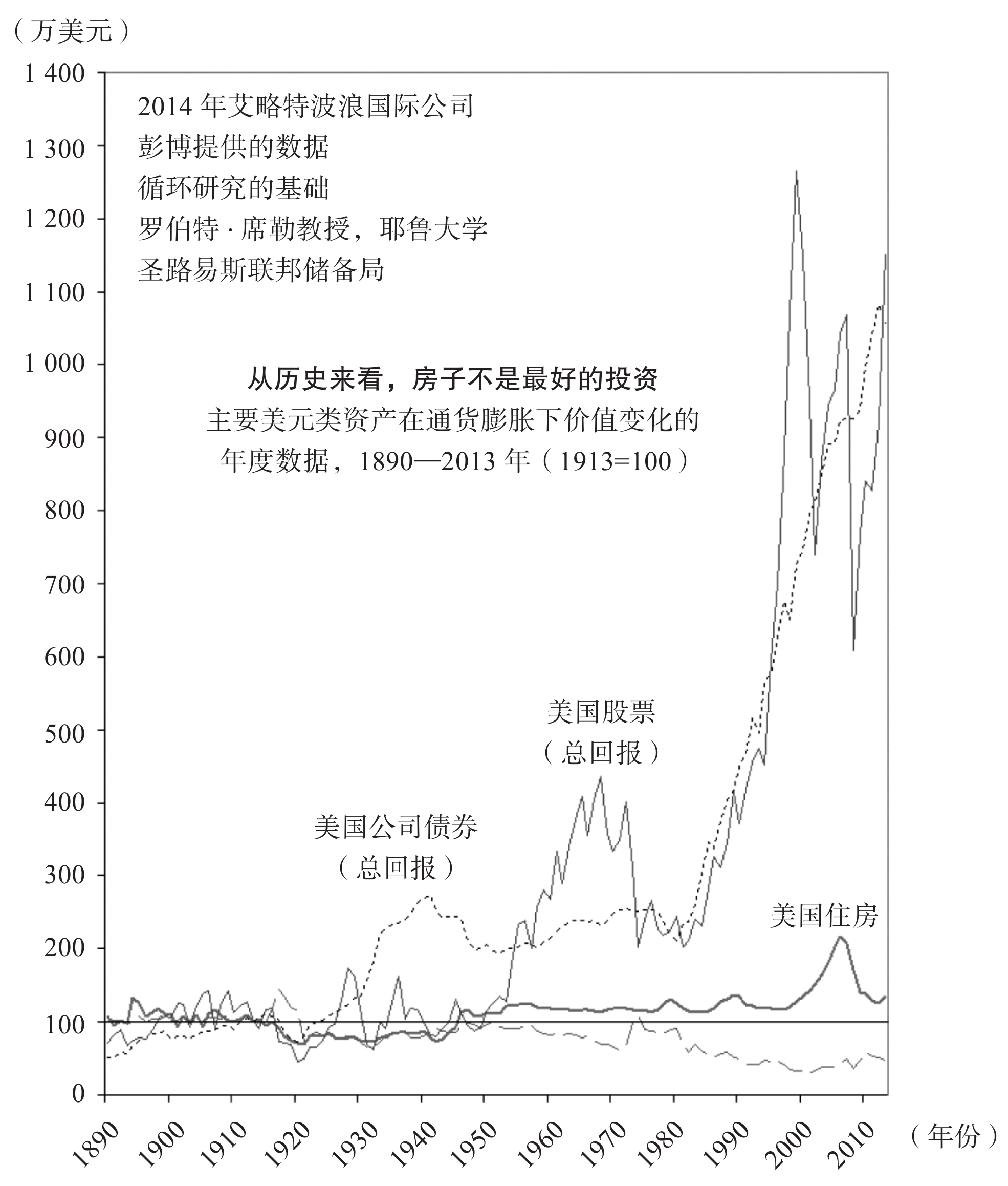
\includegraphics[width=0.7\linewidth]{image/22-3.jpg}
\caption{}\label{fig:22-3}
\end{figure}

那么，与此同时，还有哪些资产应该属于安全/安心水桶？

5.你的养老金。你有养老金吗？这个水桶就是放置养老金的好地方，美国人只有少数人有养老金，如果你是少数幸运者中的一员的话，那简直太好了。还记得波士顿大学退休研究中心主任艾丽西亚·穆勒的故事吗？她把自己的养老金变现，提前拿到了一笔钱，她觉得自己用这些钱做投资，肯定比她的前任雇主赚的投资回报率更高，而她的前任雇主就是美国联邦储备局。结果她亏得很惨，并学到了一个深刻的教训：你不要拿你一生的收入计划去冒险。现在她鼓起勇气讲出自己犯错的故事，以警告其他人。

6.年金。要是你还年轻，听说过年金这个词，你会觉得这东西对于你来说没有一点儿用。过去，买年金需要先交一大笔钱，而且你必须到一定年纪，才有资格运用年金这种投资工具。但是你会在第28章中学到，现在有些新型的年金，你也可以用来武装自己。记住，你投资的是保险产品，它能给你一份有保障的终身收入。这些年金如果收费合理、投资得当的话，类似于个人养老金，就可以作为社会养老金和企业养老金的补充。但是正如我们讨论过的那样，大多数年金的投资做得很糟糕，收取的费用又很高，还有荒谬的惩罚条款。大多数可变年金都应该加上更多的警告，要比伟哥广告上的警告更多！但是你会发现，你可以精选出来少数年金（你会在第五部分详细了解），它们非常安全，价钱也不贵，一般人都能买得起，很多专家称之为“退休收入解决方案的圣杯”。这是怎么回事？因为这种年金能让你一举两得，让你既可以享受风险/成长水桶的那种高收益，又能享有安全/安心水桶的那种高安全性。这种年金能够给你一份有保障的终身收入，而且你的投资价值从来不会下跌。

7.至少有一种人寿保险属于你的安全/安心水桶，你不要乱动它。为什么？你成家了吗？拥有它，如果你死了，你的家庭会得到照顾。拥有定期人寿保险对于大多数人来说足够了。不过，还有其他类型的人寿保险可以给你带来终身收入，而且完全免税，只要你还活着你就能领取收入！如果结构安排得当的话，这种年金还可以提供巨大的税收效率。全世界最大的公司和超级富豪一直运用这种年金投资来规避税收，这是美国税务局批准的避税方式，他们这样做了好几十年了。你一定要仔细阅读第29章，详细了解如何运用这种工具，它可能会把你实现财务目标的时间缩短1/4\textasciitilde{}1/2，具体比例取决于你的税率等级。

8.结构化票据。这种产品对于投资者来说就像工程设计一样安全。结构化票据就像是市场联结型大额存单，但是它不在美国联邦存款保险公司的承保范围之内。它是如何运作的？你借钱给一家银行（往往是全世界最大的银行），这家银行保证会把钱还给你，至到期日那一天，它还让你分享你在此期间约定的某个指数累计涨幅的一定比例［比如标准普尔500指数（减去红利），也可以是大宗商品、黄金、房地产信托基金，或者这些产品的组合］。在我写本书的时候，摩根大通公司有一个7年期的结构化票据，它有100\%的下行保护，这意味着你绝对不会损失你的原始投资本金，而且它让你分享90\%的标准普尔指数的上行收益。不要怀疑，正如你在第13章中所学到的，那些超级富豪经常用这种工具来进行投资。类型合适的结构化票据是一个非常棒的投资方式，能让你一举两得，既能分享股市上涨的收益，又不用担心承受股市下行的风险，特别是在人生的某个阶段，在你根本承担不起那些波动性风险的时候，这种结构化票据会特别适合你。

关于结构化票据，我请教了玛丽·卡拉汉·厄道斯，她是摩根大通资产管理公司的首席执行官，管理资产规模2.5万亿美元。我们俩坐下来交流时，她告诉我，结构化票据可以成为很好的投资选择，特别是对于那些经历了2008年金融危机的人来说，它最合适了。这不是什么把戏，也没有猫腻。“很多时候，人们一看结构化票据就会说‘这简直太好了，不可能是真的’。”她告诉我，“但是你需要搞明白这个产品，从头到尾地仔细了解它。你会发现，它根本没有玩什么花招，也没有玩什么小把戏，这只是市场上的一个简单的算术题……你不需要流动性的时间越久，你的钱放在市场上投资的时间就越长，自然市场付给你的钱就会更多。如果你愿意把你的钱拿出来7年不用，经过这么长的时间，你应该能够得到市场上涨的收益。”

那么结构化票据应该被归入你的安全/安心水桶吗？结构化票据的安全性取决于发行这个票据的银行。厄道斯说得非常清楚，摩根大通是世界上最大的银行，有些受托人可能会推荐加拿大皇家银行或者其他加拿大银行，因为它们得到的评级是世界最高的，是最安全的。（美国在大萧条期间倒闭的银行超过9400家，而在最近这场金融危机期间倒闭的银行接近50家，但是在加拿大没有一家银行倒闭！）所以，一如既往地，你要权衡收益和风险后，再做出投资决策。你还要留心费用和复杂的合同。我们在第13章中讲过，结构化票据可能会成为非常糟糕的产品，就像公募基金一样，如果有太多的费用附加在上面，它就会变得很糟糕。如果结构化票据的发行人的财务状况非常强健，你就不会亏掉你的本金，但是如果时机不对的话，你可能投资了相当长的时间也赚不到一分钱。所以，结构化票据更大程度上属于一种追求安全保障的投资选择。你最好先跟你的受托投资顾问好好聊一聊这种投资，看准了再下手去买，这样更加妥当。

\subsection{时间站在你这边}

上面这些内容太多了。你感觉你的脑袋快要被塞爆了，因为投资选择太多，其实不只你会这样，好多人都会。你可以轻松地搞定资产配置（并且评估你的整个投资组合），只要登录堡垒理财网就行了，或者你找自己的受托人投资顾问来帮你进行资产配置。

但是重要的是，要理解资产配置的概念，确定什么样的投资适合放到安全/安心水桶，什么样的投资适合放到风险/成长水桶，好让你的整个投资组合（就是你的这些投资选手组成的团队）可以符合你的投资收益率目标和你的风险承受能力。用这种方式，你可以继续主持大局！在每一个决策点上，你都应该想一想：“我冒的风险有多大，我保有资产的安全程度有多大？”正是这一点决定着你玩这个投资游戏会赢还是会输。

正如你看到的那样，安全/安心水桶现在面临的最大挑战是：什么才是真正安全可靠的投资？我们知道世界已经变了，即使是更加保守的储蓄者，也被迫进入愈加高风险的投资领域，这都是被低到疯狂的利率所逼的。努力追求更高的收益率很有诱惑力，特别是当股票市场快速上涨的时候。你开始想：“我可能永远也到不了我想要达到的目标了。”但是如果你愿意玩长期的投资游戏的话，你是可以做到的。（特别是如果你能找到一些投资，既能够保证收益，又不用承受损失本金的风险——你很快就会学到。）

正如滚石乐队唱的那首老歌的歌词：“时间站在你这边，财富要增长，时间来帮忙。”对于安全/安心水桶来说，时间肯定是最伟大、最宝贵的资产——即使你是在人生比较晚的阶段才开始积累财富的。毕竟，有越来越多的人能活到80多岁或者90多岁，寿命变长了，投资的时间也变长了，所以我们的投资能和我们一起慢慢变老，投资期限到了，正好也到我们晚年要花钱的时候了。如果你是“80后”“90后”“00后”，你投资游戏的时间还很长！你可以从很少的资金开始起步，让复利的力量带你到你想去的地方，复利一发挥作用，一切就容易多了。

放到安全/安心水桶里的钱，收益率比较低，但是其长期投资的结果会如何？这让我想起了一个故事。那是一个老赌徒在高尔夫球场上玩的把戏。这个赌徒报出了他的杆数：“你玩高尔夫？我刚开始打，我打得不好。你愿意玩点儿钱吗？一个洞只赌10美分？”那个对手马上同意了，说：“好，没问题！”在走向第一洞的路上，这个赌徒说：“你知道的，10美分赌得太小了，没什么意思。为了更有意思，我们把每个洞的赌金翻1倍，怎么样？”第一洞是10美分，第二洞是20美分，第三洞是40美分。到了第五洞，赌注就是1.6美元，第六洞是3.2美元。一共要打18洞，打完前6洞的机会是1/3。等他们打到第18洞的时候，你猜赌注会是多少？13107美元！一个洞赌这么大，简直是天价。这个例子说明了一旦复利发挥作用，其威力会有多么巨大。

当你用你的安全/安心水桶做投资的时候，经过较长的时间，你的投资也会发生这样的事情。你用你得到的利息再投资，经过很长一段时间之后，看起来好像没有进展，但是等你到了第13洞、第14洞、第15洞时，它就会突然爆发式增长。你看一看下面的图，这是一个指数增长的过程，会对你的财富增长发挥巨大作用。

当然，老老实实地坐在那里一动不动，对于现代人来说是一个巨大的挑战。从整个社会来看，我们都非常迷恋于马上得到回报，等着我们安全/安心水桶里的资产增值，一开始，我们的感觉好像是看着青草生长一样缓慢。正是因为这个原因，我们经常受不了诱惑，会把钱都投到第二个水桶——风险/成长水桶。但是，并不是安全/安心水桶里的每一项资产都收益率很低，像洗碗机一样无趣。如果你找到了一个很有才华又人脉很广的受托人投资顾问，他会展示给你如何从这些无聊的证券工具中选出一些好的投资工具，让你获得一个更加合理的收益率，甚至是相当不错的收益率，只要你找到合适的机会就行。

\begin{figure}[htbp]
\centering
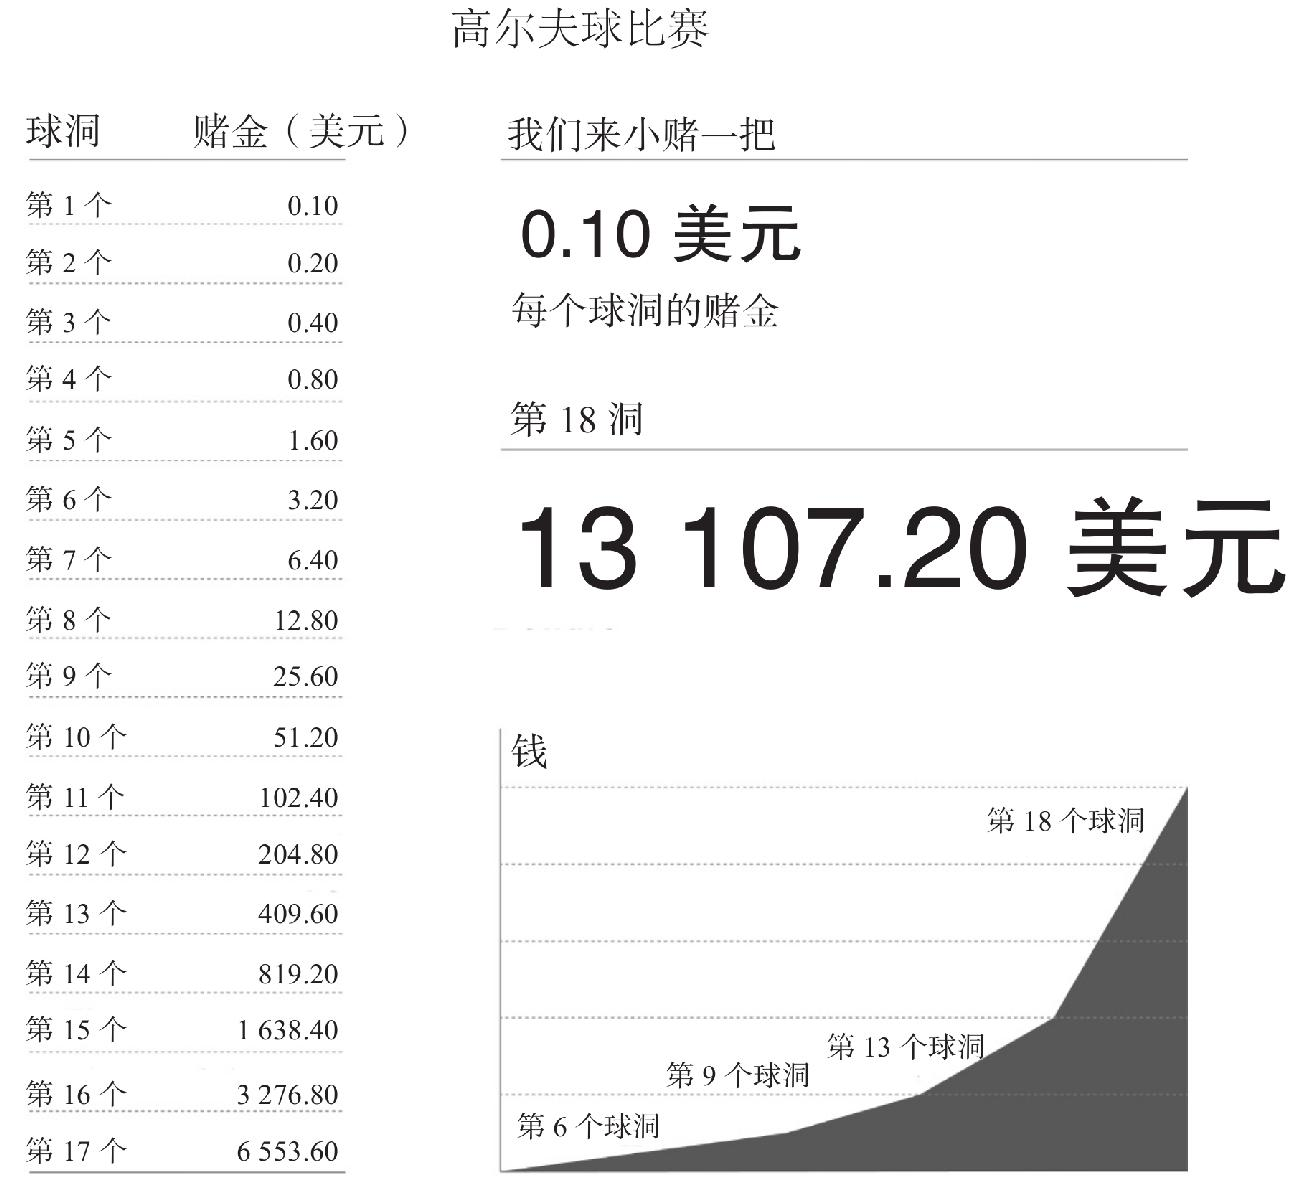
\includegraphics[width=0.78\linewidth,keepaspectratio]{image/22-4.jpg}
\caption{}\label{fig:22-4}
\end{figure}

这里只是简单举个例子，它是我的投资顾问给我找到的一个投资机会——大多数人一般不会把这种资产放到他们的安全/安心水桶里——住宅房地产贷款！

这个项目源于一个故事，一个人在加利福尼亚州的印第安维尔斯建造房子，他在财务上碰到麻烦了，不得不把这幢住宅卖给其他投资人。你听说过印第安维尔斯吗？那个地方就像比弗利山庄，是美国人均收入最高的地方之一。城市很美，气候宜人，城市周围都是高尔夫球场和风景区——在这个地方买套房子或者投资度假屋，那简直太棒了。一个投资公司买了这个人的房子，还买了几十套类似的房产，所以它需要很多现金，但是这家公司不需要持有这些资产很长时间，因为它会修缮一下这些房子，再重新把房子快速卖掉，好让资金保持良好的周转，这家投资公司需要投资者提供一些短期贷款，作为交换，它可以把公司持有的这些房产的第一信托契约转让给投资者。

你听说过第一信托契约吗？如果你拥有一套房子，借了一笔抵押贷款，金融机构贷款给你买这套房子，然后你给它打了一张借条，正式的说法是签订贷款合同，并承诺到期归还本金，按照一定的收益率支付利息。可是，如果你不能遵守承诺，没能按期还款，那么拥有这个抵押权或者信托契约的机构就有权强迫你卖掉房子，然后继续收取利息，直到一个新的持有人接手。作为一个投资者，我寻找途径在安全的环境下获得最大化的回报——第一信托契约的结构安排合理，能够完美地实现我的这个目标。

我和我的投资顾问发现，那家房地产投资公司把提供第一信托契约的那套印第安维尔斯的房子作为抵押，想得到100万美元、一年支付10\%利息的贷款。这家公司既愿意一个投资者投资100万美元，也能接受最多25个人平均每个人贷款4万美元。最终，我决定一个人投资100万美元。你也许会说：“这笔交易真是非常棒！你那100万美元资金只需要锁定一年就能赚到10万美元。但是，托尼，你知道你的风险是什么吗？”这正是我要做很多研究的原因。这套房子，有两家有资质的机构做过价值评估，我知道，按照现在的情况，这套房子价值200万美元。如果我贷款给那家公司100万美元，这笔贷款和房屋价值之比就是1∶2，对不对？即使公司违约了，我那100万美元也是安全的，因为这套房产本身就值200万美元。

这是一个非常棒的交易，但是我也买了一些面积更小的房子的信托契约。比如，我发现，在美国中西部有一套供初次购房者购买的房子，价值8万美元。如果我能够用4万美元得到抵押权，相当于抵押贷款和房屋价值之比为1∶2，我就可以做这笔投资了。其实这和印第安维尔斯那套房子的交易一模一样，只不过后者规模更大一些。于是，我决定做这笔投资，我把这笔投资放进了我的安全/安心水桶。

好了，我觉得你肯定会说：“等等，托尼！如果房地产市场下跌了，怎么办？这种投资难道不应该归于风险/成长水桶吗？”

这个问题问得很好，因为我们刚刚经历了一场有史以来最糟糕的房地产大崩盘。从表面来看，似乎你应该把这笔房地产投资放在风险/成长水桶里。但是这也正是我觉得这笔房地产投资很安全的原因。2008年房地产市场跌到了谷底，整个世界都崩溃了，房地产的价格在美国大部分地区下跌了30\%\textasciitilde{}40\%，但也有更严重的地方，比如拉斯维加斯、凤凰城、迈阿密的部分区域，房价跌幅超过了50\%，但是所有这些地方的房价在泡沫破裂之前，都有过巨大的涨幅。印第安维尔斯并没有经历这么大的泡沫——2008—2010年房价下跌了31\%（远远低于50\%），单个年度房价的最大跌幅只有13.6\%（这发生在2008—2009年）。我们的钱拿出去贷给别人，只有一年时间。所以，既然印第安维尔斯的房地产市场在2008年那样的环境下都没有暴跌50\%，那么今年它也不可能出现这样的情况。

这也正是为什么我要把这笔投资归到安全/安心水桶里。在房地产这个领域做投资，你务必小心谨慎。但是房地产投资并不一定收益率低得让人根本提不起兴趣（有时房地产收益率会相当不错，能达到8\%\textasciitilde{}10\%，而大多数人在安全/安心水桶里的投资能有1\%\textasciitilde{}4\%的收益率，就令人相当满意了），但前提是你要做好功课。

\begin{BookQuote}
我的看法和大家不同，伊索写的龟兔赛跑的那个寓言，是卖给乌龟读者群的。兔子根本没有空儿读这种东西。

\hfill ——安妮塔·布鲁克
\end{BookQuote}

\begin{BookQuote}
无聊来自无聊的头脑。

\hfill ——《内心的挣扎》（金属乐队）
\end{BookQuote}

现在，如果同一家公司给我提供12\%的收益率，让我投资那套价值200万美元的房产，因为我得到的收益率更高，所以这家公司希望我能贷款给它的资金更多，不是100万美元，而是150万美元。我投资还是不投资呢？在这种情况下贷款金额与房屋价值的比例提高到75\%——很明显，我得到了更高的收益，代价是承担更高的风险。这意味着，如果市场下跌25\%甚至更多，我可能会亏一些钱。不是万一，而是可能。所以，如果我愿意承担更大的风险来追求更高的收益，这件事就值得我考虑一下。但是我不会把这种投资放进我的安全/安心水桶里，这属于另一个水桶，你很快会在下一章了解到。这个水桶应该贴上一个黄色警告的标签，你摆弄这个水桶的时候必须戴上隔热手套，因为如果你的处理方式不正确，我敢保证它会把你的手烧焦。但是如果你对这个水桶处理的方式有效而且得当，它可以大大加速你通向财务自由的旅程。

现在，你能明白为什么资产配置是一种艺术，而不是一种科学了。安全的概念完全是主观的，有些人觉得无论什么事情都不安全，有些人能够容忍冒那么一点风险。所以，你需要根据个人的基本情况，具体看待每一笔投资的风险。

资产配置真正的好处在于，你估算出合适的资产配置比例：你的钱有多大比例用来保证安全，多大比例你愿意拿去冒险追求更高的收益，好让你的财富增长得更快。在投资上，资产配置决定你成功还是失败，所以你认为自己应该把多大比例的资产放进你的安全/安心水桶——只做安全的投资？1/3？1/2？2/3？如果你不能确保把相当大一部分你辛辛苦苦赚来的钱放在安全的投资上，你可能将来在财务上会大难临头。反过来，要是你把太多的钱放在这个安全/安心水桶里，就会显著地拖累你的财富增长。我们如何找到适当的平衡点？这正是我们努力的目标。既然我们已经锁定了安全的基础，现在是时候真正进入比赛了。

下面是一篇对债券的概述，它就像快速记录的简短笔记。我们来简要介绍一下债券的主要类型，因为债券对于你的安全/安心水桶来说可能是个非常重要的投资，所以这份债券概述很值得你仔细读一下。如果现在读你觉得不太合适，没关系，你只要记住这里有一份简单介绍债券主要类型的参考资料就行了，你可以跳过去直奔下一章。保持那股冲劲。我们正在奔向更大的风险，可能也会有更大的收益。

\subsection{债券简介}

\begin{BookQuote}
绅士们喜欢债券。

\hfill ——安德鲁·梅隆（纽约梅隆银行创始人）
\end{BookQuote}

不久之前，大家都认为债券是最安全、最可靠的投资形式。在超级富豪的投资组合里，债券是大炮，对于普通投资者来说，债券是你安全/安心水桶的奠基石。但是债券最近几年名声很差，这也很自然。美国政府把利率压得非常低，低得离谱。有些发行债券的公司、城市，甚至国家摇摇欲坠——几乎要破产了，购买这些债券对于所有人来说不再是好买卖了。

但是大多数专家仍然认为，在投资组合中，债券还是非常重要的组成部分。（事实上，债券是投资组合的基础，有了债券，你才能组建一个令人震惊的投资组合，让你在所有的经济气候中都能获得良好的收益，你会在第26章中进一步了解。）所以，让我们了解一下债券有哪些基本类型，看一看它们都有哪些优点可以被利用，也看一看它们有哪些缺点需要我们注意。

\textbf{美国国债。}很多投资专家，包括耶鲁大学的资产配置奇才戴维·斯文森，都认为，世界上最安全的债券就是历史悠久的美国国债，因为它们有美国政府提供的完全信用担保。戴维告诉我：“有了美国国债，就像给投资组合装了铁锚。”但是因为这些债券非常安全，不可能违约，所以美国国债的收益率就低很多。和其他那些不太安全的债券一样，国债也会受到外部事件的冲击，发生价格波动。所以突然之间，你原来觉得债券是一个防弹型投资，但它就在你面前变成炸弹爆炸了。

美国国债有4种不同的类型（它们有不同的名字，按照它们距离到期日时间的长短来命名）。

1.短期国债：这些国债是美国政府借的债，期限不超过12个月。短期国债是短期债券指数基金和货币市场基金投资组合的根基所在。

2.中期国债：期限为1\textasciitilde{}10年，提供固定利率（称为息票）。你可以每隔6个月收到一次利息收益。

3.长期国债：和中期国债一样，但期限长得多，10\textasciitilde{}30年。

4.美国通货膨胀保值国债：首创于1997年，这些美国政府通货膨胀保值国债可以保护你避免受到通货膨胀猛增的打击。当你买了通货膨胀保值国债之后，你的本金（就是票面价值）会随着消费价格指数的变化而上下波动，消费价格指数就是反映通货膨胀变化的统计指标——你一年两次收到的利息也会随之变化。所以如果你买了10000美元的通货膨胀保值国债，年利率1.5\%，如果消费价格指数在6个月里没有变化，那么你的债券“票面价值”就会保持不变，你还会得到150美元的利息，但是，如果生活成本，也就是消费价格指数上升了2\%，你的债券也会随之升值2\%，现在的价值是10200美元，那么你一年两次收到的利息也随之升值2\%，利息变为153美元。所以，如果你持有很多通货膨胀保值国债，恰巧又发生了很多次通货膨胀，那么你赚的钱会大大增加！下表展示了通货膨胀保值国债是如何运作的。

% 来源：OEBPS/Text/Section0001_split_004.xhtml → image_8703d05a32b74548b92a0ceb4f7b05b6.jpg
\begin{longtable}{@{}C{\dimexpr 0.07000\linewidth-1.71429\tabcolsep\relax}C{\dimexpr 0.09000\linewidth-1.71429\tabcolsep\relax}C{\dimexpr 0.15000\linewidth-1.71429\tabcolsep\relax}C{\dimexpr 0.16000\linewidth-1.71429\tabcolsep\relax}C{\dimexpr 0.18000\linewidth-1.71429\tabcolsep\relax}C{\dimexpr 0.21000\linewidth-1.71429\tabcolsep\relax}C{\dimexpr 0.14000\linewidth-1.71429\tabcolsep\relax}@{}}
\caption{雷蒙德·詹姆斯通货膨胀保值国债}\label{tab:22-1}\\
\toprule\noalign{\vskip 3pt}
{\heiti 年数} & {\heiti 优惠（\%）} & {\heiti 票面价值（美元）} & {\heiti 通货膨胀情况} & {\heiti 消费物价指数变化情况} & {\heiti 调整后的资本价值（美元）} & {\heiti 利息（美元）} \\
\midrule
\endfirsthead
\multicolumn{7}{r}{续表}\\[0.6em]
\toprule\noalign{\vskip 3pt}
{\heiti 年数} & {\heiti 优惠（\%）} & {\heiti 票面价值（美元）} & {\heiti 通货膨胀情况} & {\heiti 消费物价指数变化情况} & {\heiti 调整后的资本价值（美元）} & {\heiti 利息（美元）} \\
\midrule
\endhead
\bottomrule
\endfoot
\bottomrule
\endlastfoot
1 & 1.5 & 1\,000 & 通货膨胀 & +2 & 1\,020 & 15.30 \\
2 & 1.5 & 1\,020 & 通货紧缩 & −1 & 1\,010 & 15.15 \\
3 & 1.5 & 1\,010 & 通货膨胀 & +3 & 1\,040 & 15.60 \\
4 & 1.5 & 1\,040 & 通货膨胀 & +2 & 1\,060 & 15.90 \\
5 & 1.5 & 1\,060 & 通货膨胀 & +1 & 1\,070 & 16.05 \\
\end{longtable}


请注意，这种债券的价值也会向下调整。所以，我们如果进入另外一场经济衰退或者经济萧条，就可能损失一部分本金。你如果当时需要提前清算你的债券，按照当时的市值拿钱走人，就只能接受折价贴现。

基本上，如果你买的是通货膨胀保值国债，你就是在赌我们会进入一个通货膨胀的时期。这看起来可能吗？如果你不太确定（其实没有人能够百分之百地确定），你也许可以参照戴维·斯文森推荐的理想投资组合：因为利率上升的时候（通常发生在通货膨胀时期），通货膨胀保值国债会随之上涨。你可以买入同样数量的传统国债，因为传统国债正好与通货膨胀保值国债相反，在利率上涨的时候它的价格会下跌。这样双面下注的话，不管发生什么情况，你的投资价值都能得到保护。

当然，美国并不是唯一发行国债的国家，很多国家也要通过发行债券来筹集资金，维持政府部门的运作。在过去美好的日子里，其实就在几年前，有主权国家完全信用担保的债券，市场普遍认为它们是相当安全的投资选择。但是现在我们看到希腊、西班牙和其他国家都濒临违约，或者像阿根廷一样正在快速坠落，外国政府发行的国债已经成了相当危险的买卖。外国国债在通货膨胀风险面前更加脆弱。如果你买了一个外国债券，其发行货币是不太稳定的外国货币，你要把它们换成美元可能会遇到很大的麻烦。大多数投资顾问都说，还是把这些外国债券的投资留给那些专业的交易员和对冲经理好了，你最好碰都别碰。

但是有没有其他债券能够带来更好的收益率，胜过那些普通的传统国债？下面列出的一些国债类型比其他债券相对更加安全。你要了解其他人对这些类型投资前景的看法，只要看一看这些债券的信用评级就行了。这些评级是根据债券对投资者的风险水平测评进行分类的。

有几个是国际上公认的债券评级机构，比如穆迪、惠誉评级、标准普尔，它们应用特别的公式来对不同发行人进行信用评级，这有点儿像你申请汽车贷款或者万士达信用卡时对你的信用进行评级。标准普尔的债券评级，最高是AAA（代表最高水平的信心，相信这个公司或者国家不会让它发行的债券违约），接下来是BBB（属于“投资级”债券），然后是CCC，最低是D（意味着债券发行人已经违约了）。债券评级越低，发行人就需要付给债券持有人更高的利息，以补偿他们承担的更高风险。以前大家都把评级低于BBB的债券称为垃圾债券，因为这些是“低于投资级”的债券。这些债券被专业人士重新命名，避开了评级，他们只谈其收益，业内称之为“高收益债券”。

\textbf{公司债券。}公司债券是公司发行的债券，公司想要筹集资金来扩张业务、收购兼并、支付股息、弥补亏损，各种各样的原因都有。那么你应该买公司债吗？这取决于风险大小。如果你选择了错误的债券，你可能会亏掉大部分钱，甚至是全部的钱。尽管有些行业内的老牌公司，比如环球航空公司和柯达公司也都破产了。就在宣布破产一年之前，柯达公司的无担保债券，1美元的面值在市场上只能卖到14美分。但是大多数美国巨无霸公司发行的债券，市场仍然认为它们是相当安全的投资。苹果公司（信用评级AA+）一直在发行高信用评级的债券，把它们卖给饥渴的投资者，但是这些债券的利率只比美国国债高1\%左右！有些投资者，就像戴维·斯文森会说：“为什么要费事去买公司债券？你看好这些公司，就直接去买这些公司的股票好了，你可以获得比债券高得多的收益率。”

但是，如果你想在债券上寻找更高的收益率，你有很多选择。只是这些投资应该进入你的风险/成长水桶，而不是你的安全/安心水桶！比如，大多数人都想回避的所谓的垃圾债券，你必须一个一个地仔细研究，决定这些债券值不值得你冒这么大的风险买入。2014年5月，澳大利亚最大的航空公司澳洲航空公司发行了低于投资级评级的垃圾债券，8年期，发行货币是澳元，年利率7.75\%。澳洲航空公司的信用评级降低了，因为最近它出现了亏损和债务问题，但是你会因此就不考虑投资这只债券吗？或者在一个更加极端的层次上，2013年1月，就在一片极端混乱之中，有些人正在购买一年期的埃及短期国债，有担保（你可以想象一下，不稳定的政府做出的担保能有多可靠呢），年收益率14.4\%。买这样债券的家伙是在赌，美国政府和沙特阿拉伯政府肯定会出手相助，让埃及保持稳定，埃及能够按时偿付债务，不然它会破坏整个中东地区的稳定。

你追求的债券承诺的收益是不是值得你去冒债券违约的风险？在购买之前，你必须深思熟虑后，再做出这种决策。

当然，我们中很多人既没经验又没时间去做这种高水平的专业研究。一个有才华的受托人投资顾问，也是这个领域的专家，正好可以大显身手。但是也有一些美国国内和国际高收益债券指数基金，可以给你创造良好的收益，同时把风险分散到很多债券上。

\textbf{市政债券。}什么是市政债券？一个州（相当于中国的省）、市、县需要筹集资金来建设大型市政工程（排水系统、医院、公共交通），当地通过发行债券来借钱搞建设。过去，每个人都认为这些市政债券是双赢的买卖，因为市政债券支付的利息通常免缴美国联邦所得税，可能也会免缴州所得税。但是美国这些市和县发生了什么情况？加利福尼亚州的圣贝纳迪诺和斯托克顿，亚拉巴马州的杰斐逊县，底特律、芝加哥，这些地方政府要么破产了，要么是在破产的边缘，这些地方政府发行的市政债券的持有人倒霉了，将来他们可能会两手空空。他们心里肯定非常生气，当时购买债券的时候，这些市政债券看起来是绝对稳赚的买卖。他们以后再也不会这么天真了。而且，当市场利率水平下跌时，有的时候，这些债券的发行人会提前“赎回”，在债权到期日之前强行归还你的本金。你本来指望能够获得有保障的高收益率，结果一下子就没了。但是你如果认识到了这些风险，也可能找到一些非常好的投资机会，前提是你要有眼光，知道到哪里去寻找，而且市政债券的税收优势确实非常大。

这里有个案例也许对你有参考价值。我有个朋友最近买了纽约市发行的市政债券，他能够得到4\%的免税收益率。对于那些需要交纳高税收的人来说，这相当于一个7\%左右的应纳税债券［7\%×（1–40\%）=4.2\%］！为什么他不担心风险？这些债券是用纽约市政府未来的税收收入作为担保的。而如果将来纽约市政府遇到麻烦了，它有能力来提高税收，确保这只债券按期还本付息！他觉得这只债券非常好，他甚至愿意把它归入自己的安全/安心水桶！

关键是，可能会有很多的市政债券对于你来说很有投资价值，但是你需要学习很多相关的知识，多多请教注册投资顾问，或者请教其他见多识广的投资专家。这些人对某些市政债券非常内行。

要给你的投资组合选择适当的债券，以及配置适当的比例，进行适当的组合，这很不容易，你需要做很多预测的工作。你如果不想进行这么麻烦的预测工作，先锋公司创始人约翰·博格的建议是，购买一只低成本又低费用的债券指数基金，你就能够充分分散投资风险，因为这样你就会拥有债券市场的每一个组成部分。在第六部分中，你会看到博格如何把他的这个理念转化为行动，来构建他自己的投资组合。

现在我们继续前进到第二个水桶：风险更高，潜在收益率也更高。
